\documentclass[a4paper, 11pt, normalem]{article}

\usepackage{../../LaTeX-Templates/Notes}
\usepackage{subfiles}
\usepackage{adjustbox}

\title{The Little Crash Course of Particle Physics \vspace{-20pt}}
\author{Prof. Alex Lenz}
\date{\vspace{-15pt}Michaelmas 2019}
\rhead{\hyperlink{page.1}{Contents}}

\begin{document}

\maketitle

\section*{First Meeting}
\textbf{\large QED:}
\begin{align}
    \La &= \bar{\psi}(i\cancel{\p}-m)\psi - \frac14F_{\mu\nu}F^{\mu\nu} \\
    \cancel{\p} &\to \cancel{D}: D_\mu = \p_\mu - ieA_\mu \\
    F_{\mu\nu} &= \p_\mu A_\nu - \p_\nu
\end{align}

\textbf{\large Symmetry:}
\begin{align}
    \psi &\to e^{i\alpha}\psi \\
    A^\mu &\to A'^\mu = A^\mu + \p^\mu\alpha(x)
\end{align}
Known as a $U(1)$ local gauge symmetry, for EM. \\
Most accurate measurement in modern science is $(g-2)$ for the electron. 
Gone on to 5-loop now, $>10000$ diagrams to calculate that. 
\begin{table}[H]
    \centering
    \begin{tabular}{c|c|c|c}
        gauge & SU(N) & $N^2-1$ & N charges \\
        \hline
        strong & SU(3) & 8 gluons & 3 colours \\
        weak & SU(2) & $W^{+/-},Z^0$ & 2 charges \\
        (gravity) & & &
    \end{tabular}
\end{table}
\begin{align}
    \psi &\to \begin{cases} \begin{pmatrix} \psi_A \\ \psi_B \end{pmatrix} & \text{weak} \\ \begin{pmatrix} \psi_i \\ \psi_j \\ \psi_k \end{pmatrix} & \text{strong} \end{cases} & e^{i\alpha} &\to \begin{cases} e^{i\alpha_i\tau_i} & \text{weak, Pauli matrices, }i=1,2,3 \\ e^{i\alpha_i\lambda_i} & \text{strong, Gell-Mann matrices, }i=1,\dots,8 \end{cases}
\end{align}

The theoretical scattering rate of $B^- \to  K^-\mu^+\mu^-$ does not match that of experiment close enough that it can be simply down to innacuracies in experiment, so we posit a new boson, the \textit{Z'}, that could explain the difference between theory and experiment, and then we must find if such a boson can exist in harmony with the rest of the Standard Model.
\begin{equation}
    \text{\Large Exp} = 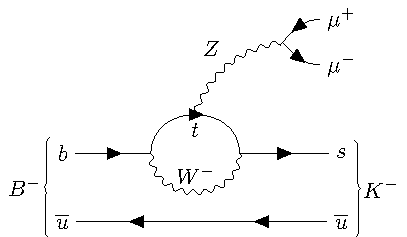
\includegraphics[raise=-20pt]{bminus.pdf} + 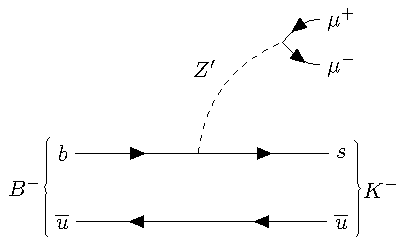
\includegraphics[raise=-20pt]{bminusprime.pdf}
\end{equation}  
Eq (7) shows the suggested sum, with the second diagram showing the new \textit{Z'} that may account for the difference. \\
For this \textit{Z'} to be the solution to the inconsistencies, it must also hold for all other couplings it could affect in the Standard Model.


\end{document}
